% Provenance (never printed): old premiere S material on the structure of the
% Earth from seismology (P and S waves, travel times, the Moho, the shadow zone
% and the core, a reference model); see sources/book2/PROVENANCE.md. Profiles
% from figdata/grade-11/prem_profiles.py, rays and travel times from
% seismic_rays.py, the refraction lines and the problem's readings from
% moho_refraction.py. Lehmann's story and portrait are told in Book 1 (g6
% inside-the-earth): recalled here, not repeated.
\chapter{भूकंपीय तरंगें पृथ्वी का भीतरी भाग प्रकट करती हैं}\label{ch:g11:seismic-structure}

8 अक्टूबर 1909 को एक भूकंप ने क्रोएशिया में ज़ाग्रेब से लगभग \qty{40}{km} दक्षिण-पूर्व में
कुपा नदी की घाटी को हिला दिया। कुछ महीने पहले आंद्रिया
मोहोरोविचिच ने ज़ाग्रेब मौसमविज्ञान वेधशाला में एक नया भूकंपलेखी यंत्र लगाया था,
और उसने पूरी घटना दर्ज की। फिर उन्होंने दूसरी
वेधशालाओं से उनके अभिलेख माँगे और 41 स्टेशनों के अभिलेख इकट्ठे किए। अधिक दूर के
स्टेशनों के अभिलेखों पर उन्हें कुछ अप्रत्याशित मिला: दो
अलग-अलग \omterm{def:g11:seismic-structure:body-waves}{P तरंगें}, पहले एक दुर्बल और फिर एक अधिक प्रबल, जहाँ एक ही होनी
चाहिए थी। तरंगों की उस जोड़ी से उन्होंने निष्कर्ष निकाला कि भूपर्पटी के नीचे की चट्टान
भिन्न है, और उन्होंने उस सीमा की गहराई मापी। यह अध्याय दिखाता है कि
भूकंप की तरंगों के पहुँचने के समय पृथ्वी की परतें कैसे प्रकट करते हैं:
भूपर्पटी का आधार, क्रोड और उसका द्रव बाहरी भाग, और
पूरा भीतरी भाग, गहराई-दर-गहराई।
% ledger: herak:kupa-1909, srl:mohorovicic, geotech:moho-1909, kayal:pn-sn

\begin{recall}
भूकंप पृथ्वी के भीतर एक बिंदु पर शुरू होता है, जो भूकंप-मूल है; उसके ठीक ऊपर
सतह का बिंदु अधिकेंद्र है। भूकंपमापी ज़मीन के काँपने को दर्ज करता है,
और परिमाण भूकंप का आकार मापता है (पुस्तक 1,
कक्षा 7)। पृथ्वी में भूपर्पटी, प्रावार और क्रोड हैं; क्रोड का एक द्रव
बाहरी भाग और एक ठोस भीतरी भाग है। भूकंप की तरंगें मुख्यतः दो प्रकार की होती हैं,
अधिक तेज़ \omterm{def:g11:seismic-structure:body-waves}{P तरंगें} और अधिक धीमी \omterm{def:g11:seismic-structure:body-waves}{S तरंगें}, और \omterm{def:g11:seismic-structure:body-waves}{S तरंगें} द्रव को पार नहीं कर सकतीं
(पुस्तक 1, कक्षा 6)। दो पदार्थों की सीमा पार करने वाली तरंग, जिनमें
वह चालों $v_1$ और $v_2$ से चलती है, अपवर्तित होती है:
$\sin i_1/v_1 = \sin i_2/v_2$, जहाँ कोण सीमा के
अभिलंब से मापे जाते हैं (स्नेल का नियम; भौतिकी की पुस्तकें)।
\end{recall}

\section{भूकंपीय तरंगें और यात्रा-काल}

\subsection{काय तरंगों के दो प्रकार}

भूकंप सभी दिशाओं में तरंगें भेजता है। कुछ सतह के अनुदिश चलती हैं;
दूसरी, काय तरंगें, पृथ्वी के भीतर से होकर चलती हैं, और वही
उसे प्रकट करती हैं।

\begin{definition}[P तरंग; S तरंग]\label{def:g11:seismic-structure:body-waves}
\emph{P तरंग}\index{P तरंग} ऐसी भूकंपीय तरंग है जो चट्टान को बारी-बारी से संपीडित
करती और खींचती है: चट्टान उसी दिशा के अनुदिश आगे-पीछे चलती है जिसमें
तरंग चलती है। यह ठोसों, द्रवों और गैसों को पार करती है, और यह
सबसे तेज़ भूकंपीय तरंग है, इसलिए सबसे पहले पहुँचती है। \emph{S तरंग}\index{S तरंग}
चट्टान का अपरूपण करती है: चट्टान उस दिशा के समकोण पर चलती है जिसमें
तरंग चलती है। यह केवल ठोसों को पार करती है, और P तरंग के बाद पहुँचती है।
\end{definition}
% ledger: kayal:p-s

द्रव बहता है और आकार-परिवर्तन का कोई प्रतिरोध नहीं करता, इसलिए वह
अपरूपण को आगे नहीं बढ़ा सकता: इसीलिए \omterm{def:g11:seismic-structure:body-waves}{S तरंगें} द्रव की सतह पर रुक जाती हैं। अधिकांश
चट्टानों में \omterm{def:g11:seismic-structure:body-waves}{P तरंग} \omterm{def:g11:seismic-structure:body-waves}{S तरंग} से लगभग $\sqrt 3 \approx 1.7$ गुना तेज़ चलती है।
ऊपरी भूपर्पटी में \omterm{def:g11:seismic-structure:body-waves}{P तरंग} लगभग \qty{5.8}{km/s} से और \omterm{def:g11:seismic-structure:body-waves}{S तरंग}
लगभग \qty{3.2}{km/s} से चलती है; भूपर्पटी के ठीक नीचे वे लगभग
\qty{8.1}{km/s} और \qty{4.5}{km/s} तक पहुँचती हैं।
% ledger: kayal:p-s, kayal:outer-core-liquid, data:prem (vp_surface 5.8, vs_surface 3.2,
% vp_upper_mantle 8.11, vs_upper_mantle 4.49 in figdata/grade-11/prem_profiles.py)

\begin{omfigure}
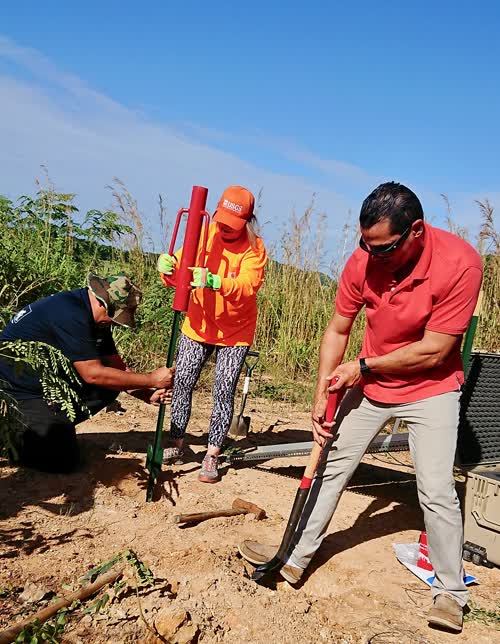
\includegraphics[width=0.5\linewidth]{images/book2/g11-usgs-seismometer.jpg}

{\small पोर्टो रिको भूकंपीय नेटवर्क और USGS के भूकंपविज्ञानी 10 जनवरी
2020 को दक्षिण-पश्चिमी पोर्टो रिको में एक अस्थायी भूकंपमापी लगाते हुए।
फ़ोटो: थॉमस प्रैट, USGS (सार्वजनिक डोमेन)।}
\end{omfigure}
% ledger: photo:g11-seismometer

\subsection{यात्रा-काल वक्र}

किसी भूकंप से दूर के किसी स्टेशन की दूरी एक
कोण के रूप में मापी जाती है: पृथ्वी के केंद्र पर अधिकेंद्र और स्टेशन के बीच का कोण $\Delta$,
यानी \emph{अधिकेंद्री दूरी}\index{अधिकेंद्री दूरी}। इसका एक
अंश सतह के अनुदिश $\qty{111.2}{km}$ है।
% ledger: earth:Rmean

\begin{definition}[यात्रा-काल; यात्रा-काल वक्र]\label{def:g11:seismic-structure:travel-time}
किसी स्टेशन पर किसी भूकंपीय तरंग का \emph{यात्रा-काल}\index{यात्रा-काल} वह
समय है जो वह भूकंप-मूल से स्टेशन तक जाने में लेती है। किसी तरंग का
\emph{यात्रा-काल वक्र}\index{यात्रा-काल वक्र} स्टेशन की अधिकेंद्री दूरी के सापेक्ष
उसके यात्रा-काल का आलेख है।
\end{definition}

स्टेशन वह समय दर्ज करता है जब हर तरंग पहुँचती है; जब भूकंप का
समय ज्ञात हो, तो अंतर ही \omterm{def:g11:seismic-structure:travel-time}{यात्रा-काल} है। हज़ारों स्टेशनों द्वारा दर्ज हज़ारों
भूकंपों ने \omterm{def:g11:seismic-structure:travel-time}{यात्रा-काल वक्र} बहुत सटीकता से दिए हैं। चित्र में वक्र
\cref{sec:g11:seismic-structure:model} के \omterm{def:g11:seismic-structure:reference-model}{संदर्भ पृथ्वी मॉडल} से परिकलित हैं, और
बिंदु वास्तविक भूकंपों में प्रेक्षित \omterm{def:g11:seismic-structure:travel-time}{यात्रा-काल} हैं: दोनों हर जगह दो प्रतिशत के
भीतर मेल खाते हैं, और प्रायः एक या दो सेकंड के भीतर।

\begin{omfigure}
\begin{tikzpicture}
\begin{axis}[omrecord, width=0.84\linewidth, height=6.4cm, xmin=0, xmax=180, ymin=0, ymax=30,
  xtick={0,20,...,180}, ytick={0,5,...,30},
  xlabel={अधिकेंद्री दूरी $\Delta$ (अंश)}, ylabel={यात्रा-काल (मिनट)},
  tick label style={font=\small}, label style={font=\small}, clip=false]
% computed in figdata/grade-11/seismic_rays.py; ledger: data:prem, auspass:surftim
\addplot[omDef, line width=0.9pt] table[x=delta_deg, y=t_min] {figdata/out/grade-11-seismic_rays-ttp.dat};
\addplot[omProp, line width=0.9pt] table[x=delta_deg, y=t_min] {figdata/out/grade-11-seismic_rays-tts.dat};
\addplot[omDef, line width=0.9pt, densely dashed] table[x=delta_deg, y=t_min] {figdata/out/grade-11-seismic_rays-ttpkp.dat};
\addplot[omDef!55, line width=0.9pt, densely dotted] table[x=delta_deg, y=t_min] {figdata/out/grade-11-seismic_rays-ttpkikp.dat};
\addplot[only marks, mark=*, mark size=1.5pt, black] table[x=delta_deg, y=p_min] {figdata/out/grade-11-seismic_rays-observed.dat};
\addplot[only marks, mark=*, mark size=1.5pt, black, unbounded coords=discard] table[x=delta_deg, y=s_min] {figdata/out/grade-11-seismic_rays-observed.dat};
\node[font=\small, text=omProp, anchor=south east] at (axis cs:68,21.2) {S};
\node[font=\small, text=omDef, anchor=north west] at (axis cs:72,11.2) {P};
\node[font=\small, text=omDef, anchor=south, align=center] at (axis cs:158,23.2) {क्रोड से होकर\\P};
\fill[black!10] (axis cs:98.5,0) rectangle (axis cs:143.8,3.2);
\node[font=\scriptsize, align=center] at (axis cs:121.1,1.6) {कोई सीधी P नहीं};
\end{axis}
\end{tikzpicture}

{\small सतह पर हुए भूकंप से \omterm{def:g11:seismic-structure:body-waves}{P तरंगों} (नीला) और \omterm{def:g11:seismic-structure:body-waves}{S तरंगों} (नारंगी) के \omterm{def:g11:seismic-structure:travel-time}{यात्रा-काल वक्र},
\omterm{def:g11:seismic-structure:reference-model}{संदर्भ पृथ्वी मॉडल} से परिकलित; डैश
और बिंदुदार वक्र वे \omterm{def:g11:seismic-structure:body-waves}{P तरंगें} हैं जिन्होंने क्रोड पार किया है (बिंदुदार: आंतरिक
क्रोड)। काले बिंदु: प्रेक्षित \omterm{def:g11:seismic-structure:travel-time}{यात्रा-काल}। लगभग \ang{99} और
\ang{144} के बीच कोई \omterm{def:g11:seismic-structure:body-waves}{P तरंग} सीधे नहीं पहुँचती (छायांकित)।}
\end{omfigure}

S वक्र P वक्र की अपेक्षा अधिक तेज़ी से चढ़ता है, इसलिए दोनों आगमनों के बीच की
देरी दूरी के साथ बढ़ती है। इससे एक ही अभिलेख से भूकंप की दूरी
मिल जाती है।

\begin{method}[S--P देरी से भूकंप की दूरी]\label{met:g11:seismic-structure:distance}
\begin{enumerate}
  \item अभिलेख पर पहली \omterm{def:g11:seismic-structure:body-waves}{P तरंग} और पहली \omterm{def:g11:seismic-structure:body-waves}{S
        तरंग} का समय पढ़िए; उनका अंतर S--P देरी है।
  \item \omterm{def:g11:seismic-structure:travel-time}{यात्रा-काल वक्रों} पर (या उनकी तालिका में) वह
        अधिकेंद्री दूरी ढूँढिए जिस पर S वक्र P वक्र से उतनी ही देरी
        ऊपर है।
  \item आवश्यक हो तो $\qty{111.2}{km}$ प्रति अंश से किलोमीटर में बदलिए।
\end{enumerate}
तीन स्टेशनों से अधिकेंद्र वह बिंदु है जो तीनों से सही
दूरी पर है।
\end{method}

\begin{example}[\ang{60} दूर एक भूकंप]\label{ex:g11:seismic-structure:sp}
\ang{60} पर प्रेक्षित \omterm{def:g11:seismic-structure:travel-time}{यात्रा-काल} P के लिए \qty{608}{s} और S के लिए \qty{1101}{s} हैं,
\ang{50} पर \qty{536}{s} और \qty{967}{s}। इसलिए जो स्टेशन \omterm{def:g11:seismic-structure:body-waves}{P तरंग} के \qty{493}{s}
(8~मिनट 13~सेकंड) बाद \omterm{def:g11:seismic-structure:body-waves}{S तरंग} दर्ज करता है, वह
अधिकेंद्र से \ang{60} पर है: लगभग $60 \times 111.2 \approx
\qty{6670}{km}$। \ang{50} पर देरी केवल \qty{431}{s} होती।
\end{example}
% ledger: auspass:surftim

\begin{omfigure}
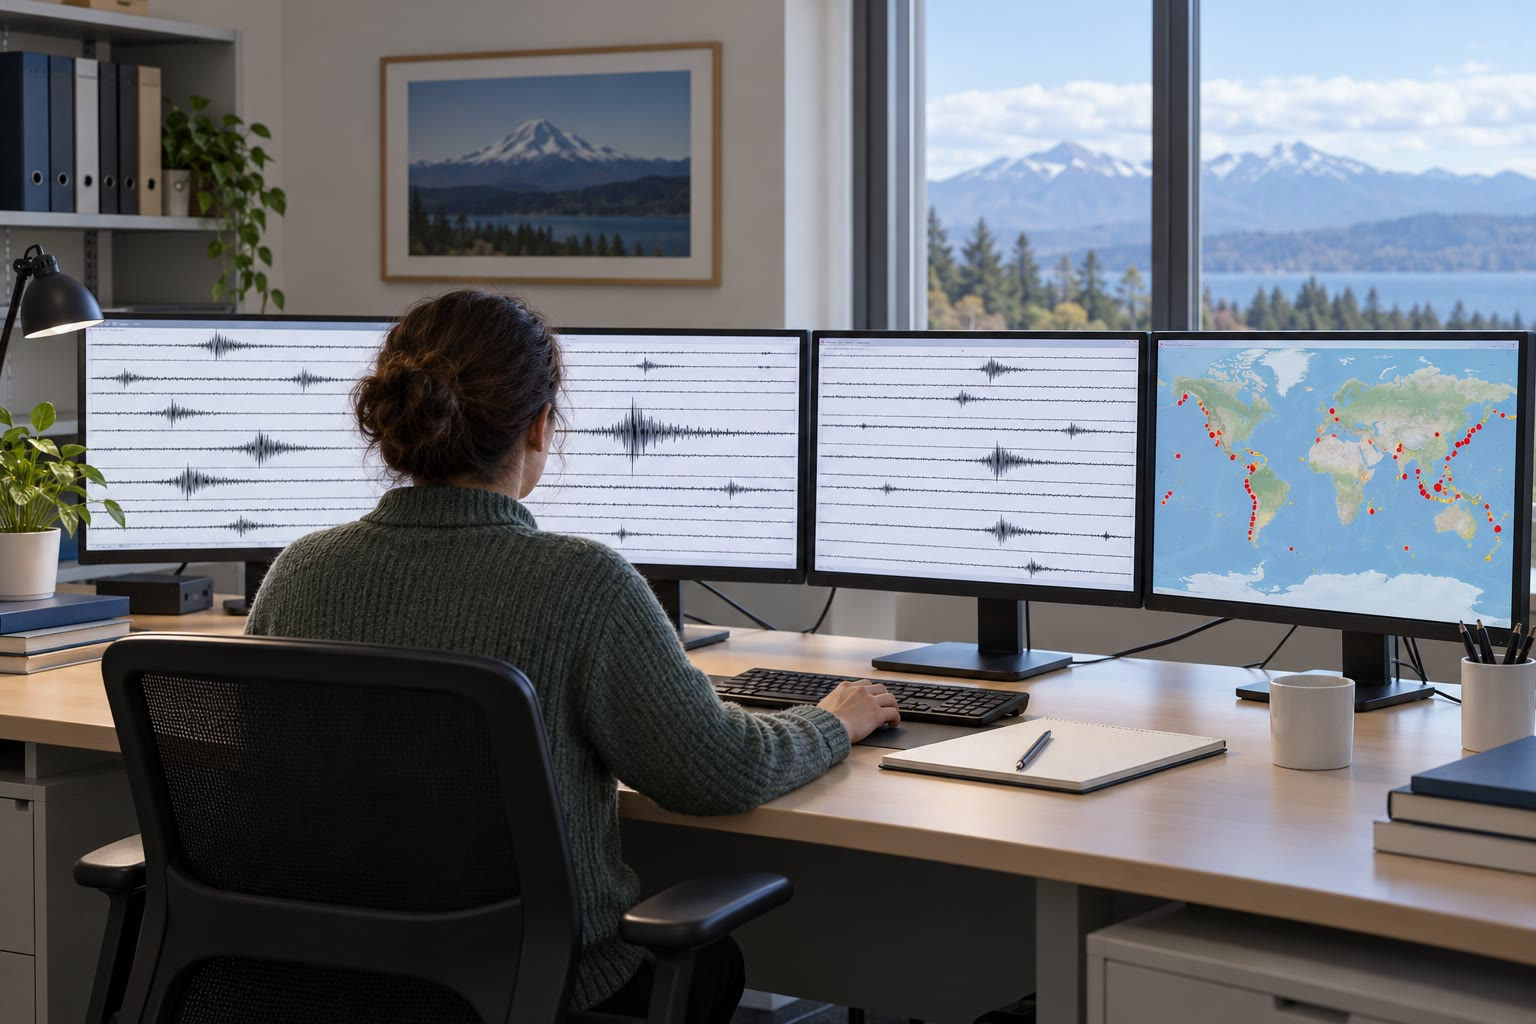
\includegraphics[width=0.66\linewidth]{images/book2/ai/g11-seismology-observatory.jpg}

{\small किसी भूकंपविज्ञान वेधशाला में अनेक स्टेशनों के अभिलेख
साथ-साथ दिखाए जाते हैं, और वे जिन भूकंपों की स्थिति निर्धारित करते हैं, वे विश्व-मानचित्र पर आलेखित किए जाते हैं
(AI चित्रण)।}
\end{omfigure}

\section{अपवर्तन और मोहो}\label{sec:g11:seismic-structure:moho}

\subsection{सीमा के अनुदिश दौड़ने वाली तरंग}

पृथ्वी के भीतर भूकंपीय तरंगों की चाल गहराई के साथ बदलती है, अधिकतर
धीरे-धीरे, पर कुछ स्थानों पर एकाएक।

\begin{definition}[भूकंपीय असांतत्य]\label{def:g11:seismic-structure:discontinuity}
\emph{भूकंपीय असांतत्य}\index{भूकंपीय असांतत्य} पृथ्वी के भीतर ऐसा पृष्ठ
है जिसके आर-पार भूकंपीय तरंगों की चाल एकाएक बदल जाती है ---
तरंगों की लंबाई से बहुत कम मोटाई में।
\end{definition}

असांतत्य पर तरंग का एक भाग परावर्तित होता है और एक भाग अपवर्तित। मोटाई $h$ की
एक परत लीजिए जिसमें \omterm{def:g11:seismic-structure:body-waves}{P तरंगें} $v_1$ से चलती हैं, और जो ऐसी परत के ऊपर है
जिसमें वे अधिक तेज़ हैं, $v_2 > v_1$। ऊर्ध्वाधर से कोण $i$ पर नीचे जाती किरण
कोण $r$ पर अपवर्तित होती है, जो $\sin r = (v_2/v_1)\sin
i$ से मिलता है: वह ऊर्ध्वाधर से दूर मुड़ती है। जब $\sin i$ का मान $v_1/v_2$ तक पहुँचता है, तो
अपवर्तित किरण ठीक सीमा के अनुदिश चलती है। कोण
\[
  i_c, \qquad \sin i_c = \frac{v_1}{v_2},
\]
\emph{क्रांतिक कोण}\index{क्रांतिक कोण} है। \omterm{ex:g11:seismic-structure:sp}{क्रांतिक कोण} पर अपवर्तित
तरंग तेज़ परत के शीर्ष के अनुदिश चाल $v_2$ से चलती है,
और चलते हुए वह ऊपरी परत में तरंगें वापस ऊपर भेजती है, सभी कोण
$i_c$ पर: वे सतह पर \emph{शीर्ष तरंग}\index{शीर्ष तरंग} के रूप में पहुँचती हैं।

\begin{omfigure}
\begin{tikzpicture}[x=0.05cm, y=0.05cm, font=\footnotesize, >={Stealth[length=4pt]}]
% geometry from figdata/grade-11/moho_refraction.py: v1 6.2, v2 8.1, h 30 km, ic 49.9 deg
  \fill[omLithGranite!45] (-10,0) rectangle (215,-30);
  \fill[omLithPeridotite!45] (-10,-30) rectangle (215,-48);
  \draw[line width=0.6pt] (-10,0) -- (215,0);
  \draw[line width=0.9pt] (-10,-30) -- (215,-30);
  \node[anchor=west, align=left] at (218,-15) {भूपर्पटी\\$v_1 = \qty{6.2}{km/s}$};
  \node[anchor=west, align=left] at (218,-39) {प्रावार\\$v_2 = \qty{8.1}{km/s}$};
  \node[anchor=east] at (215,-26) {मोहो};
  % source and station
  \fill[omDef] (0,0) circle (1.6);
  \node[anchor=south] at (0,1.5) {भूकंप};
  \draw[fill=white] (197,0) -- (203,0) -- (200,5) -- cycle;
  \node[anchor=south] at (200,5) {स्टेशन};
  % direct wave
  \draw[->, omProp, line width=0.8pt] (2,-2) -- (196,-2);
  \node[anchor=south, text=omProp] at (100,0.3) {सीधी तरंग, चाल $v_1$};
  % head wave
  \draw[omDef, line width=0.9pt] (0,0) -- (35.7,-30);
  \draw[->, omDef, line width=0.9pt] (35.7,-30) -- (100,-30);
  \draw[omDef, line width=0.9pt] (100,-30) -- (164.3,-30) -- (200,0);
  \node[anchor=north, text=omDef] at (100,-31) {मोहो के अनुदिश $v_2$ से};
  \foreach \x in {50,70,90,110,130,150} {
    \draw[->, omDef!60, densely dashed] (\x,-30) -- ++(25.5,21.5);
  }
  % critical angle
  \draw[black!60, densely dotted] (35.7,-30) -- (35.7,-8);
  \draw[black!70] (35.7,-18) arc[start angle=90, end angle=130.05, radius=12];
  \node[anchor=south east] at (33,-16) {$i_c$};
  % thickness and critical distance
  \draw[<->] (-6,0) -- (-6,-30);
  \node[anchor=east] at (-7,-15) {$h$};
\end{tikzpicture}

{\small सीधी तरंग और \omterm{ex:g11:seismic-structure:sp}{शीर्ष तरंग} (पैमाने पर: भूपर्पटी \qty{30}{km}
मोटी)। \omterm{ex:g11:seismic-structure:sp}{शीर्ष तरंग} \omterm{ex:g11:seismic-structure:sp}{क्रांतिक कोण} $i_c$ पर नीचे जाती है, प्रावार के शीर्ष के
अनुदिश दौड़ती है और $i_c$ पर वापस ऊपर आती है; \omterm{def:g11:seismic-structure:moho}{मोहो} पर अपने पूरे मार्ग के अनुदिश
वह सतह की ओर तरंगें ऊपर भेजती है (डैश)। वह $2h\tan i_c$ से
निकट किसी स्टेशन तक नहीं पहुँचती, जो यहाँ लगभग \qty{71}{km} है।}
\end{omfigure}

\begin{proposition}[शीर्ष तरंग का यात्रा-काल]\label{prop:g11:seismic-structure:head-wave}
सतह पर स्थित स्रोत के लिए, दूरी $x \ge 2h\tan i_c$ पर स्थित स्टेशन
\omterm{ex:g11:seismic-structure:sp}{शीर्ष तरंग} इतने समय बाद प्राप्त करता है:
\[
  t(x) = \frac{x}{v_2} + \frac{2h\cos i_c}{v_1}.
\]
इसका \omterm{def:g11:seismic-structure:travel-time}{यात्रा-काल वक्र} ढाल $1/v_2$ की एक सरल रेखा है, जो पीछे
बढ़ाने पर समय-अक्ष को \emph{अंतःखंड काल}\index{अंतःखंड काल}
$t_i = 2h\cos i_c/v_1$ पर काटती है।
\end{proposition}

\begin{proof}
किरण लंबाई $h/\cos i_c$ की एक तिरछी भुजा पर नीचे जाती है, जो
क्षैतिज रूप से $h\tan i_c$ आगे बढ़ती है; ऊपर लौटते हुए भी यही होता है। बीच में वह
सीमा के अनुदिश $x - 2h\tan i_c$ चलती है। समय है
\[
  t = \frac{2h}{v_1\cos i_c} + \frac{x - 2h\tan i_c}{v_2}
    = \frac{x}{v_2} + \frac{2h}{v_1\cos i_c} - \frac{2h\sin i_c}{v_2\cos i_c}.
\]
चूँकि $1/v_2 = \sin i_c/v_1$, अंतिम दो पद मिलकर
$\frac{2h}{v_1\cos i_c}\,(1 - \sin^2 i_c) = \frac{2h\cos i_c}{v_1}$ बनाते हैं।
\end{proof}

सीधी तरंग $x/v_1$ के बाद पहुँचती है: उसका वक्र मूल-बिंदु से होकर जाने वाली
एक रेखा है, जो शीर्ष-तरंग की रेखा से अधिक खड़ी है। स्रोत के पास सीधी तरंग
पहले आती है; दूर, \omterm{ex:g11:seismic-structure:sp}{शीर्ष तरंग}, जो मार्ग का अधिकांश भाग अधिक चाल से
दौड़ी है, उससे आगे निकल जाती है।

\begin{proposition}[अतिक्रमण दूरी]\label{prop:g11:seismic-structure:crossover}
\omterm{ex:g11:seismic-structure:sp}{शीर्ष तरंग} \emph{अतिक्रमण
दूरी}\index{अतिक्रमण दूरी} के आगे सीधी तरंग से पहले पहुँचती है, जो यह है:
\[
  x_c = 2h\sqrt{\frac{v_2 + v_1}{v_2 - v_1}}.
\]
\end{proposition}

\begin{proof}
दोनों एक साथ तब पहुँचती हैं जब $x/v_1 = x/v_2 + 2h\cos i_c/v_1$, यानी
$x\,(v_2 - v_1)/(v_1 v_2) = 2h\cos i_c/v_1$, इसलिए $x = 2h\cos i_c\,v_2/(v_2 -
v_1)$। अब $\cos i_c = \sqrt{1 - v_1^2/v_2^2} = \sqrt{(v_2 - v_1)(v_2 +
v_1)}/v_2$, अतः $x = 2h\sqrt{(v_2 + v_1)(v_2 - v_1)}/(v_2 - v_1) =
2h\sqrt{(v_2 + v_1)/(v_2 - v_1)}$। इसके आगे \omterm{ex:g11:seismic-structure:sp}{शीर्ष तरंग}, जिसकी रेखा
कम खड़ी है, पहले पहुँचती है।
\end{proof}

\begin{omfigure}
\begin{tikzpicture}
\begin{axis}[omrecord, width=0.78\linewidth, height=5.6cm, xmin=0, xmax=300, ymin=0, ymax=50,
  xtick={0,50,...,300}, xlabel={अधिकेंद्र से दूरी (\unit{km})}, ylabel={यात्रा-काल (\unit{s})},
  tick label style={font=\small}, label style={font=\small}, clip=false]
% computed in figdata/grade-11/moho_refraction.py (critical_km 71.4, crossover_km 164.6, intercept_s 6.23)
\addplot[omProp, line width=0.9pt] table[x=x, y=tdirect] {figdata/out/grade-11-moho_refraction-model.dat};
\addplot[omDef, line width=0.9pt, restrict x to domain=71:300] table[x=x, y=thead] {figdata/out/grade-11-moho_refraction-model.dat};
\addplot[omDef, densely dashed, restrict x to domain=0:72] table[x=x, y=thead] {figdata/out/grade-11-moho_refraction-model.dat};
\draw[black!50, densely dotted] (axis cs:164.6,0) -- (axis cs:164.6,26.5);
\node[font=\scriptsize, anchor=north] at (axis cs:164.6,0) {$x_c$};
\fill (axis cs:0,6.23) circle (1.5pt);
\draw[black!60] (axis cs:0.8,6.6) -- (axis cs:6,12);
\node[font=\scriptsize, anchor=south west, inner sep=1pt] at (axis cs:5,12) {$t_i = \qty{6.2}{s}$};
\node[font=\small, text=omProp, anchor=south east] at (axis cs:250,41) {सीधी तरंग};
\node[font=\small, text=omDef, anchor=north west] at (axis cs:235,33) {शीर्ष तरंग};
\end{axis}
\end{tikzpicture}

{\small पिछले चित्र की भूपर्पटी के लिए सीधी तरंग और \omterm{ex:g11:seismic-structure:sp}{शीर्ष तरंग} के
\omterm{def:g11:seismic-structure:travel-time}{यात्रा-काल}। शीर्ष-तरंग की रेखा, पीछे बढ़ाने पर (डैश), समय-अक्ष को
\omterm{prop:g11:seismic-structure:head-wave}{अंतःखंड काल} पर काटती है; \omterm{prop:g11:seismic-structure:crossover}{अतिक्रमण दूरी} $x_c \approx
\qty{165}{km}$ के आगे \omterm{ex:g11:seismic-structure:sp}{शीर्ष तरंग} पहले पहुँचती है।}
\end{omfigure}

\subsection{भूपर्पटी का आधार}

\begin{definition}[मोहो]\label{def:g11:seismic-structure:moho}
\emph{मोहोरोविचिच असांतत्य}\index{मोहोरोविचिच असांतत्य}, या
\emph{मोहो}\index{मोहो}, भूपर्पटी के आधार पर स्थित \omterm{def:g11:seismic-structure:discontinuity}{भूकंपीय असांतत्य} है,
जहाँ \omterm{def:g11:seismic-structure:body-waves}{P तरंगों} की चाल अधिक से अधिक लगभग \qty{7}{km/s} से उछलकर
लगभग \qty{8}{km/s} हो जाती है, जो सबसे ऊपरी प्रावार की चाल है।
\end{definition}
% ledger: kayal:pn-sn, data:prem (6.8 -> 8.11 at 24.4 km)

\begin{history}[मोहोरोविचिच और दो P तरंगें, 1909]
आंद्रिया मोहोरोविचिच (1857--1936) ने 1909 के भूकंप के अभिलेखों पर पाया
कि एक निश्चित दूरी के आगे --- सामान्यतः 100 और
\qty{150}{km} के बीच --- एक दुर्बल, अधिक तेज़ \omterm{def:g11:seismic-structure:body-waves}{P तरंग} प्रबल \omterm{def:g11:seismic-structure:body-waves}{P तरंग} से पहले पहुँचती थी।
उन्होंने इसे ऐसी तरंग के रूप में समझाया जो भूपर्पटी के नीचे की अधिक तेज़ चट्टान से होकर
चली थी। उन्होंने दोनों तरंगों के नाम Pg (भूपर्पटी में सीधी तरंग) और Pn (प्रावार के
शीर्ष के अनुदिश \omterm{ex:g11:seismic-structure:sp}{शीर्ष तरंग}) रखे, \omterm{def:g11:seismic-structure:body-waves}{S तरंगों} के लिए भी यही किया, और
दोनों परतों की चालें और उनके बीच की सीमा की गहराई निकाली।
Pn तरंग लगभग \qty{8.0}{km/s} से चलती है, जो सबसे ऊपरी
प्रावार की चाल है। उनके 1910 के शोधपत्रों ने सिद्ध किया कि भूपर्पटी और प्रावार
भिन्न हैं; वह सीमा उनका नाम धारण करती है।
\end{history}
% ledger: kayal:pn-sn, srl:mohorovicic

\begin{method}[यात्रा-काल आरेख से मोहो की गहराई]\label{met:g11:seismic-structure:moho}
\begin{enumerate}
  \item पहले आगमन के समयों को अधिकेंद्र से दूरी के सापेक्ष
        आलेखित कीजिए।
  \item सीधी तरंग की रेखा (मूल-बिंदु से होकर) और \omterm{ex:g11:seismic-structure:sp}{शीर्ष तरंग} की
        रेखा खींचिए; उनकी ढालें $1/v_1$ और $1/v_2$ हैं।
  \item शीर्ष-तरंग की रेखा को पीछे समय-अक्ष तक बढ़ाइए: वह उसे
        \omterm{prop:g11:seismic-structure:head-wave}{अंतःखंड काल} $t_i$ पर काटती है।
  \item $\sin i_c = v_1/v_2$ के साथ, भूपर्पटी की मोटाई
        $h = \dfrac{v_1\,t_i}{2\cos i_c}$ है।
\end{enumerate}
\end{method}

\begin{example}[\qty{30}{km} मोटी भूपर्पटी]\label{ex:g11:seismic-structure:moho}
$v_1 = \qty{6.2}{km/s}$ और $v_2 = \qty{8.1}{km/s}$ के साथ, $\sin i_c = 0.765$,
$i_c \approx \ang{49.9}$ और $\cos i_c \approx 0.644$। \qty{6.23}{s} का
\omterm{prop:g11:seismic-structure:head-wave}{अंतःखंड काल} $h = 6.2 \times 6.23/(2 \times 0.644) \approx
\qty{30}{km}$ देता है। \omterm{ex:g11:seismic-structure:sp}{शीर्ष तरंग} सतह पर पहली बार
$2h\tan i_c \approx \qty{71}{km}$ पर पहुँचती है और
$x_c = 60\sqrt{14.3/1.9} \approx \qty{165}{km}$ के आगे सीधी तरंग से आगे निकल जाती है।
\end{example}
% values computed in figdata/grade-11/moho_refraction.py (ic_deg 49.9, critical_km 71.4, crossover_km 164.6)

इस ढंग से पूरे संसार में मापने पर \omterm{def:g11:seismic-structure:moho}{मोहो} महासागरों की तली से केवल लगभग
\qty{5}{km} नीचे मिलता है। महाद्वीपों के नीचे वह औसतन लगभग
\qty{41}{km} नीचे है: जहाँ भूपर्पटी खिंची है वहाँ लगभग \qty{30}{km},
पर्वत-पट्टियों के नीचे \qty{45}{km} से अधिक, और सबसे ऊँची श्रेणियों के नीचे लगभग
\qty{100}{km} तक। भूपर्पटी एक पतली खाल है: \qty{41}{km} भी
पृथ्वी की त्रिज्या के एक प्रतिशत से कम है।
% ledger: usgs:crust-thickness, cm95:crust, kayal:discontinuities

\section{क्रोड}

\subsection{मुड़ने वाली किरणें}

प्रावार में भूकंपीय तरंगों की चाल गहराई के साथ बढ़ती है। नीचे जाने वाली
किरण अधिकाधिक तेज़ चट्टान पार करती है और, स्नेल के नियम के अनुसार, हर चरण पर
ऊर्ध्वाधर से थोड़ी और दूर मुड़ती है: उसका मार्ग वक्र होकर वापस
सतह की ओर ऊपर मुड़ जाता है। किरण जितनी गहराई पर मुड़ती है, भूकंप से उतनी ही दूर
वह वापस ऊपर आती है। चित्र ऐसी किरणें दिखाता है, जो
\omterm{def:g11:seismic-structure:reference-model}{संदर्भ पृथ्वी मॉडल} की चालों से परिकलित हैं।

\begin{omfigure}
\begin{tikzpicture}
\begin{axis}[width=0.66\linewidth, height=0.66\linewidth, axis equal image, hide axis,
  xmin=-1.18, xmax=1.18, ymin=-1.18, ymax=1.2, clip=false]
% computed in figdata/grade-11/seismic_rays.py; ledger: data:prem
\fill[omLithPeridotite!25] (axis cs:0,0) circle [radius=1];
\fill[omSea!45] (axis cs:0,0) circle [radius=0.5462];
\fill[omSea!80] (axis cs:0,0) circle [radius=0.1917];
\addplot[black, line width=0.6pt, domain=0:360, samples=181] ({cos(x)}, {sin(x)});
\addplot[black!60, line width=0.4pt, domain=0:360, samples=181] ({0.5462*cos(x)}, {0.5462*sin(x)});
\addplot[black!60, line width=0.4pt, domain=0:360, samples=91] ({0.1917*cos(x)}, {0.1917*sin(x)});
\addplot[omDef, line width=0.6pt] table {figdata/out/grade-11-seismic_rays-praysmantle.dat};
\addplot[omDef!70!black, line width=0.6pt] table {figdata/out/grade-11-seismic_rays-prayscore.dat};
\addplot[omProp, line width=0.6pt] table {figdata/out/grade-11-seismic_rays-srays.dat};
% P shadow zone: 98.5 to 143.8 degrees from the source (right); S beyond 102.7 (left)
\addplot[black!80, line width=3pt, domain=-53.8:-8.5, samples=40] ({1.04*cos(x)}, {1.04*sin(x)});
\addplot[omProp!60, line width=3pt, domain=192.7:270, samples=40] ({1.04*cos(x)}, {1.04*sin(x)});
\fill[omDef] (axis cs:0,1) circle (2pt);
\node[font=\footnotesize, anchor=south] at (axis cs:0,1.04) {भूकंप};
\node[font=\footnotesize, anchor=west, align=left] at (axis cs:1.07,-0.42) {कोई सीधी P नहीं\\(\ang{99}--\ang{144})};
\node[font=\footnotesize, anchor=east, align=right] at (axis cs:-1.07,-0.62) {\ang{103} से आगे\\कोई सीधी S नहीं};
\node[font=\footnotesize, text=omDef, anchor=south west] at (axis cs:0.55,0.8) {P};
\node[font=\footnotesize, text=omProp, anchor=south east] at (axis cs:-0.55,0.8) {S};
\node[font=\scriptsize] at (axis cs:-0.5,-0.62) {प्रावार};
\node[font=\scriptsize] at (axis cs:-0.3,0.2) {बाह्य क्रोड};
\draw[black!70] (axis cs:-0.1,-0.06) -- (axis cs:-0.26,-0.22);
\node[font=\scriptsize, anchor=north east, inner sep=1pt] at (axis cs:-0.24,-0.22) {आंतरिक क्रोड};
\end{axis}
\end{tikzpicture}

{\small पृथ्वी के शीर्ष पर हुए भूकंप से किरणें, संदर्भ मॉडल की
चालों से परिकलित। दाएँ: प्रावार में मुड़ने वाली P किरणें, लगभग
\ang{99} तक, और क्रोड पार करके लगभग \ang{144} के आगे निकलने वाली P किरणें;
बीच में कोई P किरण सीधे नहीं पहुँचती। बाएँ: S किरणें, जो
प्रावार में मुड़ती हैं; कोई भी द्रव बाह्य क्रोड पार नहीं करती, और कोई सीधी \omterm{def:g11:seismic-structure:body-waves}{S तरंग}
लगभग \ang{103} के आगे नहीं पहुँचती।}
\end{omfigure}

\subsection{छाया क्षेत्र और द्रव बाह्य क्रोड}

1906 में भूकंपविज्ञानी ओल्डहैम ने देखा कि भूकंप से पृथ्वी की दूर की
ओर दर्ज \omterm{def:g11:seismic-structure:body-waves}{P तरंगें} अपेक्षित समयों की तुलना में देर से पहुँचती थीं,
और एक केंद्रीय क्रोड का प्रस्ताव रखा जिसमें वे अधिक धीरे चलती हैं।
1912 में गुटेनबर्ग ने दिखाया कि \omterm{def:g11:seismic-structure:body-waves}{P तरंगें} दूरियों की एक पूरी पट्टी तक,
लगभग \ang{105} और \ang{143} के बीच, नहीं पहुँचतीं, और \ang{143} के ठीक आगे प्रबल
आगमन होते हैं; 1914 में उन्होंने क्रोड का ऊपरी सिरा \qty{2900}{km} नीचे रखा।
% ledger: kayal:discontinuities, kayal:shadow

\begin{definition}[छाया क्षेत्र]\label{def:g11:seismic-structure:shadow-zone}
किसी भूकंपीय तरंग का \emph{छाया क्षेत्र}\index{छाया क्षेत्र} अधिकेंद्री दूरियों का
वह परिसर है जहाँ तक वह तरंग किसी भूकंप से सीधे नहीं पहुँच सकती,
क्योंकि क्रोड उसे दूर मोड़ देता है या रोक देता है।
\end{definition}

किरणें इसे समझाती हैं। क्रोड के ठीक ऊपर मुड़ने वाली P किरणें
भूकंप से लगभग \ang{100} पर वापस ऊपर आती हैं। थोड़ी अधिक खड़ी जाने वाली किरण
क्रोड में प्रवेश करती है, जहाँ P चाल एकाएक \qty{13.7}{km/s} से गिरकर
लगभग \qty{8.1}{km/s} हो जाती है: स्नेल के नियम के अनुसार वह ऊर्ध्वाधर की \emph{ओर} मुड़ती है,
क्रोड पार करती है और बहुत दूर, लगभग \ang{144} के आगे, निकलती है। प्रावार में मुड़ने वाली
कोई P किरण और क्रोड पार करने वाली कोई P किरण बीच में नहीं उतरती।
संदर्भ मॉडल में P \omterm{def:g11:seismic-structure:shadow-zone}{छाया क्षेत्र} \ang{98.5} से
\ang{143.8} तक है, जो गुटेनबर्ग के \ang{105}--\ang{143} के निकट है।
% ledger: kayal:shadow, data:prem (vp_above_cmb 13.72, vp_below_cmb 8.06); computed in
% figdata/grade-11/seismic_rays.py (shadow_start_deg 98.5, shadow_end_pkp_deg 143.8)

\omterm{def:g11:seismic-structure:body-waves}{S तरंगें} और अधिक बताती हैं। कोई \omterm{def:g11:seismic-structure:body-waves}{S तरंग} बाह्य क्रोड पार नहीं करती: बाह्य क्रोड
अपरूपण तरंगें नहीं ले जाता, इसलिए वह द्रव है। परिणामस्वरूप, संदर्भ मॉडल में कोई \omterm{def:g11:seismic-structure:body-waves}{S तरंग}
लगभग \ang{103} के आगे सीधे नहीं पहुँचती --- पृथ्वी की पूरी
दूर की ओर।
% ledger: kayal:outer-core-liquid; computed in figdata/grade-11/seismic_rays.py (s_direct_max_deg 102.7)

\begin{definition}[क्रोड--प्रावार सीमा; आंतरिक-क्रोड सीमा]\label{def:g11:seismic-structure:core}
\emph{क्रोड--प्रावार सीमा}\index{क्रोड--प्रावार सीमा} ठोस प्रावार और
द्रव बाह्य क्रोड के बीच का \omterm{def:g11:seismic-structure:discontinuity}{भूकंपीय असांतत्य} है, \qty{2891}{km} की
गहराई पर; वहाँ P चाल लगभग \qty{13.7}{km/s} से गिरकर
लगभग \qty{8.1}{km/s} हो जाती है, और \omterm{def:g11:seismic-structure:body-waves}{S तरंगें} रुक जाती हैं। \emph{आंतरिक-क्रोड
सीमा}\index{आंतरिक-क्रोड सीमा}, \qty{5150}{km} की गहराई पर,
द्रव बाह्य क्रोड को ठोस आंतरिक क्रोड से अलग करती है; वहाँ P चाल
लगभग \qty{10.4}{km/s} से उछलकर लगभग \qty{11.0}{km/s} हो जाती है।
\end{definition}
% ledger: data:prem, prem:cmb, prem:icb (Book 3 rows); values in figdata/grade-11/prem_profiles.py

\omterm{def:g11:seismic-structure:shadow-zone}{छाया क्षेत्र} पूरी तरह शांत नहीं है: उसमें दुर्बल \omterm{def:g11:seismic-structure:body-waves}{P तरंगें} पहुँचती हैं। इंगे
लेहमान ने 1936 में उन्हें एक ठोस आंतरिक क्रोड से समझाया जिसमें \omterm{def:g11:seismic-structure:body-waves}{P तरंगें}
अधिक तेज़ चलती हैं (पुस्तक 1, कक्षा 6)। किरणें दिखाती हैं कि कैसे। आंतरिक क्रोड तक पहुँचने वाली
P किरण वहाँ ऊर्ध्वाधर से दूर मुड़ती है जहाँ चाल उछलकर बढ़ती है, जैसे
\omterm{def:g11:seismic-structure:moho}{मोहो} पर, और क्रोड से जल्दी बाहर निकल आती है: संदर्भ मॉडल में
आंतरिक क्रोड से होकर जाने वाली किरणें लगभग \ang{121} से आगे सतह पर पहुँचती हैं, \omterm{def:g11:seismic-structure:shadow-zone}{छाया
क्षेत्र} के भीतर (\omterm{def:g11:seismic-structure:travel-time}{यात्रा-काल} चित्र का बिंदुदार वक्र)।
% ledger: nbi:lehmann-1936 (Book 1 row), kayal:lehmann; computed in
% figdata/grade-11/seismic_rays.py (pkikp_min_deg 121.4)

\section{एक संदर्भ पृथ्वी मॉडल}\label{sec:g11:seismic-structure:model}

एक साथ रखने पर कई मिलियन \omterm{def:g11:seismic-structure:travel-time}{यात्रा-काल} हर गहराई पर P और \omterm{def:g11:seismic-structure:body-waves}{S तरंगों} की चाल
देते हैं। उनकी चालें चट्टान और उसके घनत्व पर निर्भर करती हैं, और
पृथ्वी का कुल द्रव्यमान उसका औसत घनत्व निर्धारित करता है; ये मिलकर
हर गहराई पर घनत्व भी देते हैं।
% ledger: data:prem, prem:constraints (Book 3 row)

\begin{definition}[संदर्भ पृथ्वी मॉडल]\label{def:g11:seismic-structure:reference-model}
\emph{संदर्भ पृथ्वी मॉडल}\index{संदर्भ पृथ्वी मॉडल} गहराई के सापेक्ष
\omterm{def:g11:seismic-structure:body-waves}{P तरंगों} की चाल, \omterm{def:g11:seismic-structure:body-waves}{S तरंगों} की चाल और घनत्व की एक तालिका है, जो
हर दिशा में एक-सी है, और जिसे भूकंपीय तरंगों के प्रेक्षित \omterm{def:g11:seismic-structure:travel-time}{यात्रा-कालों} से और
पृथ्वी के द्रव्यमान से मेल खाने के लिए चुना गया है।
\end{definition}

सबसे अधिक प्रयुक्त प्रारंभिक \omterm{def:g11:seismic-structure:reference-model}{संदर्भ पृथ्वी मॉडल} (PREM) है, जिसे
ए॰~एम॰~ज़िवोन्स्की और डी॰~एल॰~एंडरसन ने 1981 में प्रकाशित किया। इस
अध्याय की किरणें और \omterm{def:g11:seismic-structure:travel-time}{यात्रा-काल} इसी से परिकलित किए गए: उदाहरण के लिए, \ang{60} पर P \omterm{def:g11:seismic-structure:travel-time}{यात्रा-काल}
\qty{607}{s} आता है, जबकि प्रेक्षित \qty{608}{s} है।
% ledger: data:prem, auspass:surftim; computed in figdata/grade-11/seismic_rays.py (p_60_s 607.2)

\begin{omfigure}
\begin{tikzpicture}
\begin{axis}[omrecord, width=0.86\linewidth, height=6.2cm, xmin=0, xmax=6371, ymin=0, ymax=14.5,
  xtick={0,1000,...,6000}, ytick={0,2,...,14}, scaled x ticks=false,
  xticklabel style={/pgf/number format/1000 sep={\,}},
  xlabel={गहराई (\unit{km})}, ylabel={चाल (\unit{km/s}) या घनत्व (\unit{g/cm^3})},
  tick label style={font=\small}, label style={font=\small}, clip=false]
% computed in figdata/grade-11/prem_profiles.py; ledger: data:prem
\addplot[omDef, line width=0.9pt] table[x=depth, y=vp] {figdata/out/grade-11-prem_profiles-profile.dat};
\addplot[omProp, line width=0.9pt] table[x=depth, y=vs] {figdata/out/grade-11-prem_profiles-profile.dat};
\addplot[black, line width=0.9pt, densely dashed] table[x=depth, y=rho] {figdata/out/grade-11-prem_profiles-profile.dat};
\foreach \d in {670,2891,5149.5} {\edef\temp{\noexpand\draw[black!40, densely dotted] (axis cs:\d,0) -- (axis cs:\d,14.5);}\temp}
\node[font=\scriptsize, anchor=south, align=center] at (axis cs:2891,14.5) {क्रोड--प्रावार\\सीमा};
\node[font=\scriptsize, anchor=south, align=center] at (axis cs:5149.5,14.5) {आंतरिक-क्रोड\\सीमा};
\node[font=\scriptsize, anchor=south] at (axis cs:670,14.5) {\qty{670}{km}};
\node[font=\small, text=omDef, anchor=south] at (axis cs:1800,12.4) {P चाल};
\node[font=\small, text=omProp, anchor=south] at (axis cs:1800,7.0) {S चाल};
\node[font=\small, anchor=north] at (axis cs:1800,4.5) {घनत्व};
\node[font=\scriptsize, align=center] at (axis cs:4000,1.9) {S तरंगें नहीं:\\द्रव};
\end{axis}
\end{tikzpicture}

{\small प्रारंभिक \omterm{def:g11:seismic-structure:reference-model}{संदर्भ पृथ्वी मॉडल} (ज़िवोन्स्की और एंडरसन, 1981) में गहराई के सापेक्ष
P और \omterm{def:g11:seismic-structure:body-waves}{S तरंगों} की चालें और घनत्व। बिंदुदार
रेखाएँ \omterm{def:g11:seismic-structure:moho}{मोहो} के नीचे के मुख्य असांतत्य अंकित करती हैं; \omterm{def:g11:seismic-structure:moho}{मोहो} इतना
उथला है कि इस पैमाने पर नहीं दिखता।}
\end{omfigure}

मॉडल को ऊपर से पढ़ने पर:
\begin{itemize}
  \item भूपर्पटी, जिसमें P चालें 5.8 से \qty{6.8}{km/s} हैं, \omterm{def:g11:seismic-structure:moho}{मोहो} पर समाप्त होती है
        (इस औसत मॉडल में \qty{24.4}{km});
  \item प्रावार में चालें गहराई के साथ बढ़ती हैं, छोटे एकाएक
        उछालों के साथ, जिनमें सबसे बड़े \qty{400}{km} और \qty{670}{km} के पास हैं;
  \item \qty{2891}{km} पर S चाल शून्य हो जाती है और P चाल
        \qty{5}{km/s} से अधिक गिरती है: द्रव बाह्य क्रोड;
  \item \qty{5150}{km} पर \omterm{def:g11:seismic-structure:body-waves}{S तरंगें} फिर से होती हैं: ठोस आंतरिक क्रोड,
        जिसकी त्रिज्या \qty{1220}{km} है।
\end{itemize}
% ledger: data:prem (discontinuities in figdata/grade-11/prem_profiles.py)

घनत्व भूपर्पटी में \qty{2.6}{g/cm^3} से बढ़कर प्रावार के आधार पर
\qty{5.6}{g/cm^3} हो जाता है, फिर क्रोड के शीर्ष पर उछलकर
\qty{9.9}{g/cm^3} हो जाता है और केंद्र पर \qty{13.1}{g/cm^3} तक
पहुँचता है। पूरे मॉडल का माध्य घनत्व \qty{5.5}{g/cm^3} है, जो
भूपर्पटी की चट्टानों का दुगुना है: गहरा भीतरी भाग, और सबसे बढ़कर क्रोड,
सतह की अपेक्षा कहीं अधिक घने पदार्थ से बना है। क्रोड पृथ्वी के द्रव्यमान का लगभग
एक-तिहाई रखता है।
% ledger: data:prem, prem:cmb, prem:centre (Book 3 rows); computed in
% figdata/grade-11/prem_profiles.py (mean_density 5.52; core mass fraction 0.32)

\section{अभ्यास}

\begin{exercise}[$\star$]\label{exo:g11:seismic-structure:1}
\omterm{def:g11:seismic-structure:body-waves}{P तरंगों} और \omterm{def:g11:seismic-structure:body-waves}{S तरंगों} के बीच दो अंतर बताइए। भूकंपमापी पहले
किसे दर्ज करता है, और क्यों?
\end{exercise}

\begin{exercise}[$\star$]\label{exo:g11:seismic-structure:2}
एक स्टेशन किसी अधिकेंद्र से \ang{40} पर है। सतह के अनुदिश मापने पर वह
कितनी दूर है? किसी अधिकेंद्र से \qty{8900}{km} दूर का स्टेशन
कितने अंश दूर है?
\end{exercise}

\begin{exercise}[$\star$]\label{exo:g11:seismic-structure:3}
\ang{40} पर प्रेक्षित \omterm{def:g11:seismic-structure:travel-time}{यात्रा-काल} P के लिए \qty{456}{s} और
S के लिए \qty{822}{s} हैं। उन्हें मिनटों और सेकंडों में बदलिए, और S--P
देरी बताइए।
\end{exercise}

\begin{exercise}[$\star$]\label{exo:g11:seismic-structure:4}
ऐसी भूपर्पटी, जिसमें \omterm{def:g11:seismic-structure:body-waves}{P तरंगें} \qty{6.0}{km/s} से चलती हैं, ऐसे प्रावार पर स्थित है जहाँ
वे \qty{8.0}{km/s} से चलती हैं। \omterm{ex:g11:seismic-structure:sp}{क्रांतिक कोण} परिकलित कीजिए।
\end{exercise}

\begin{exercise}[$\star$]\label{exo:g11:seismic-structure:5}
संदर्भ मॉडल में \omterm{def:g11:seismic-structure:core}{क्रोड--प्रावार सीमा} \qty{2891}{km} गहराई पर और
\omterm{def:g11:seismic-structure:core}{आंतरिक-क्रोड सीमा} \qty{5150}{km} गहराई पर है; पृथ्वी की त्रिज्या
\qty{6371}{km} है। बाह्य क्रोड की मोटाई, क्रोड की
त्रिज्या, और पृथ्वी की त्रिज्या के भिन्न के रूप में क्रोड की त्रिज्या परिकलित कीजिए।
\end{exercise}

\begin{exercise}[$\star\star$]\label{exo:g11:seismic-structure:6}
प्रेक्षित S--P देरियाँ \ang{20} पर \qty{224}{s}, \ang{30} पर \qty{298}{s},
\ang{40} पर \qty{366}{s}, \ang{50} पर \qty{431}{s} और
\ang{60} पर \qty{493}{s} हैं। एक स्टेशन \omterm{def:g11:seismic-structure:body-waves}{P तरंग} के 6~मिनट 6~सेकंड बाद
\omterm{def:g11:seismic-structure:body-waves}{S तरंग} दर्ज करता है। भूकंप कितनी दूर है, अंशों में और किलोमीटर में?
एक अकेला स्टेशन यह क्यों नहीं बता सकता कि भूकंप कहाँ है?
\end{exercise}

\begin{exercise}[$\star\star$]\label{exo:g11:seismic-structure:7}
\cref{exo:g11:seismic-structure:4} की चालों और \qty{35}{km} मोटी भूपर्पटी के साथ,
अधिकेंद्र से \qty{200}{km} दूर किसी स्टेशन पर सीधी तरंग और
\omterm{ex:g11:seismic-structure:sp}{शीर्ष तरंग} के \omterm{def:g11:seismic-structure:travel-time}{यात्रा-काल} परिकलित कीजिए। कौन-सी पहले पहुँचती है?
\end{exercise}

\begin{exercise}[$\star\star$]\label{exo:g11:seismic-structure:8}
\cref{exo:g11:seismic-structure:7} की भूपर्पटी के लिए क्रांतिक
दूरी $2h\tan i_c$ और \omterm{prop:g11:seismic-structure:crossover}{अतिक्रमण दूरी} परिकलित कीजिए। जाँचिए कि
\cref{exo:g11:seismic-structure:7} का उत्तर इससे मेल खाता है।
\end{exercise}

\begin{exercise}[$\star\star$]\label{exo:g11:seismic-structure:9}
किसी महासागर के नीचे \qty{6}{km} मोटी भूपर्पटी, जिसमें \omterm{def:g11:seismic-structure:body-waves}{P तरंगें}
\qty{6.5}{km/s} से चलती हैं, \qty{8.0}{km/s} वाले प्रावार पर स्थित है। \omterm{ex:g11:seismic-structure:sp}{क्रांतिक
कोण}, \omterm{prop:g11:seismic-structure:head-wave}{अंतःखंड काल} और \omterm{prop:g11:seismic-structure:crossover}{अतिक्रमण दूरी} परिकलित कीजिए। किसी महासागर के नीचे \omterm{def:g11:seismic-structure:moho}{मोहो} ढूँढने के लिए
स्टेशनों को किसी महाद्वीप के नीचे की अपेक्षा बहुत अधिक पास-पास क्यों होना
चाहिए?
\end{exercise}

\begin{exercise}[$\star\star$]\label{exo:g11:seismic-structure:10}
सबसे निचले प्रावार में, जहाँ वह \qty{13.7}{km/s} से चलती है, एक P किरण
\omterm{def:g11:seismic-structure:core}{क्रोड--प्रावार सीमा} से अभिलंब के साथ \ang{30} पर मिलती है। सीमा के नीचे
P चाल \qty{8.06}{km/s} है। अपवर्तित किरण का कोण परिकलित कीजिए। क्या
किरण अभिलंब की ओर मुड़ती है या उससे दूर? इसके आधार पर समझाइए कि क्रोड में प्रवेश करने वाली P
किरणें भूकंप से दूर क्यों निकलती हैं।
\end{exercise}

\begin{exercise}[$\star\star$]\label{exo:g11:seismic-structure:11}
संदर्भ मॉडल में केंद्र से होकर सीधे नीचे जाने वाली \omterm{def:g11:seismic-structure:body-waves}{P तरंग} पृथ्वी के
विपरीत बिंदु तक पहुँचने में \qty{1210}{s} लेती है। यदि वह पूरा व्यास (\qty{12742}{km})
\qty{13.7}{km/s} से, जो प्रावार के आधार पर P चाल है, तय करती, तो उसे कितना समय लगता?
ओल्डहैम ने ऐसी देरियों से क्या निष्कर्ष निकाला?
\end{exercise}

\begin{exercise}[$\star\star\star$]\label{exo:g11:seismic-structure:12}
(1) \cref{prop:g11:seismic-structure:head-wave} से दिखाइए कि भूपर्पटी की मोटाई
यह है:
\[
  h = \frac{t_i\,v_1 v_2}{2\sqrt{v_2^2 - v_1^2}}.
\]
(2) इसे $t_i = \qty{6.23}{s}$, $v_1 = \qty{6.2}{km/s}$ और
$v_2 = \qty{8.1}{km/s}$ पर लागू कीजिए।
\end{exercise}

\begin{exercise}[$\star\star\star$]\label{exo:g11:seismic-structure:13}
पृथ्वी का माध्य घनत्व \qty{5.52}{g/cm^3} है। पृथ्वी को
\qty{3480}{km} त्रिज्या और एकसमान घनत्व $\rho_c$ वाला क्रोड मानिए, जो एकसमान घनत्व \qty{4.45}{g/cm^3}
(संदर्भ मॉडल का माध्य) वाले प्रावार और भूपर्पटी के भीतर है।
(1) पृथ्वी के आयतन का कितना भाग क्रोड है? (2)
$\rho_c$ परिकलित कीजिए। (3) संदर्भ मॉडल में क्रोड के शीर्ष के घनत्व,
\qty{9.9}{g/cm^3}, से और भूपर्पटी के घनत्व से तुलना कीजिए।
\end{exercise}

\begin{exercise}[$\star\star\star$]\label{exo:g11:seismic-structure:14}
गुटेनबर्ग का P \omterm{def:g11:seismic-structure:shadow-zone}{छाया क्षेत्र} \ang{105} से \ang{143} तक फैला है। (1) सतह के अनुदिश
किलोमीटर में उसकी सीमाएँ बताइए। (2) गोले पर, किसी बिंदु से कोणीय दूरियों $a$ और $b$
के बीच का क्षेत्रफल पूरे पृष्ठ का भिन्न $(\cos a - \cos
b)/2$ है। किसी दिए हुए भूकंप से पृथ्वी की सतह के कितने भाग तक कोई
सीधी \omterm{def:g11:seismic-structure:body-waves}{P तरंग} नहीं पहुँचती? (3) हर भूकंप का अपना
\omterm{def:g11:seismic-structure:shadow-zone}{छाया क्षेत्र} क्यों होता है?
\end{exercise}

\begin{exercise}[$\star\star\star$]\label{exo:g11:seismic-structure:15}
किसी ऊँची पर्वत-श्रेणी के नीचे एक अपवर्तन-सर्वेक्षण $v_1 =
\qty{6.3}{km/s}$, $v_2 = \qty{8.1}{km/s}$ और \qty{9.5}{s} का \omterm{prop:g11:seismic-structure:head-wave}{अंतःखंड काल}
पाता है। (1) वहाँ भूपर्पटी की मोटाई परिकलित कीजिए। (2) उन्हीं चालों के साथ \qty{30}{km} मोटी
भूपर्पटी कौन-सा \omterm{prop:g11:seismic-structure:head-wave}{अंतःखंड काल} देती?
(3) महाद्वीपीय भूपर्पटी की औसत मोटाई से तुलना कीजिए।
\end{exercise}

\section{समस्या: मोहो की खोज}

\begin{problem}[{सप्ताहांत समस्या --- पंद्रह स्टेशनों से भूपर्पटी की गहराई}]
\label{pb:g11:seismic-structure:1}
% readings computed in figdata/grade-11/moho_refraction.py (part stations; invented region,
% v1 6.2, v2 8.1, h 30 km, reading errors of up to 0.1 s); ledger: kayal:pn-sn, usgs:crust-thickness
किसी महाद्वीप के नीचे बहुत कम गहराई पर एक छोटा भूकंप आता है।
अधिकेंद्र से एक सीधी रेखा पर लगाए गए पंद्रह स्टेशन पहली \omterm{def:g11:seismic-structure:body-waves}{P तरंग} के
आगमन-समय दर्ज करते हैं और, जहाँ वह पढ़ा जा सके, एक दूसरी तरंग का भी। नीचे के
पाठ्यांक कल्पित हैं, पर उसी तरह परिकलित हैं जैसे कोई वास्तविक सर्वेक्षण
उन्हें पाता, सेकंड के दसवें भाग तक। Pg वह तरंग है जो
भूपर्पटी से होकर चलती है, Pn वह जो प्रावार के शीर्ष के अनुदिश दौड़ी है।

\begin{center}
\small
\begin{tabular}{|c|c|c||c|c|c|}
\hline
दूरी (\unit{km}) & Pg (\unit{s}) & Pn (\unit{s}) & दूरी (\unit{km}) & Pg (\unit{s}) & Pn (\unit{s}) \\ \hline
20 & 3.3 & --- & 180 & 29.0 & 28.5 \\ \hline
40 & 6.5 & --- & 200 & 32.3 & 30.9 \\ \hline
60 & 9.7 & --- & 220 & --- & 33.3 \\ \hline
80 & 12.8 & 16.2 & 240 & --- & 35.8 \\ \hline
100 & 16.1 & 18.6 & 260 & --- & 38.3 \\ \hline
120 & 19.3 & 21.1 & 280 & --- & 40.8 \\ \hline
140 & 22.6 & 23.6 & 300 & --- & 43.2 \\ \hline
160 & 25.8 & 26.0 & & & \\ \hline
\end{tabular}
\end{center}

\medskip
\noindent\textbf{भाग I --- सीधी तरंग।}
\begin{enumerate}
  \item आलेख-पत्र पर Pg और Pn समयों को दूरी के सापेक्ष आलेखित कीजिए (\qty{20}{km} के लिए
        \qty{1}{cm} और \qty{5}{s} के लिए भी)। Pg बिंदु कैसे स्थित हैं?
  \item Pg रेखा मूल-बिंदु के पास से होकर क्यों जाती है?
  \item 20 और \qty{200}{km} वाले स्टेशनों का उपयोग करके Pg रेखा की ढाल
        सेकंड प्रति किलोमीटर में परिकलित कीजिए।
  \item भूपर्पटी में \omterm{def:g11:seismic-structure:body-waves}{P तरंगों} की चाल $v_1$ निकालिए।
  \item यदि भूपर्पटी आगे जारी रहती, तो Pg तरंग \qty{300}{km} वाले स्टेशन तक
        कब पहुँचती?
\end{enumerate}

\medskip
\noindent\textbf{भाग II --- अपवर्तित तरंग।}
\begin{enumerate}[resume]
  \item 100 और \qty{300}{km} वाले स्टेशनों का उपयोग करके
        Pn रेखा की ढाल और भूपर्पटी के नीचे \omterm{def:g11:seismic-structure:body-waves}{P तरंगों} की चाल $v_2$ परिकलित कीजिए।
  \item $v_2$ की तुलना मोहोरोविचिच द्वारा मापी गई Pn तरंग की चाल,
        लगभग \qty{8.0}{km/s}, से कीजिए। भूपर्पटी के नीचे कौन-सी चट्टान है?
  \item \omterm{ex:g11:seismic-structure:sp}{क्रांतिक कोण} $i_c$ परिकलित कीजिए।
  \item \qty{80}{km} से निकट कोई स्टेशन Pn तरंग दर्ज नहीं करता।
        \cref{prop:g11:seismic-structure:head-wave} का उपयोग करके समझाइए कि
        वह न्यूनतम दूरी क्यों होती है जिस पर \omterm{ex:g11:seismic-structure:sp}{शीर्ष तरंग} दर्ज की जा सकती है।
  \item 80 और \qty{160}{km} के बीच Pn, Pg के बाद पहुँचती है। फिर भी वह
        दर्ज क्यों होती है?
\end{enumerate}

\medskip
\noindent\textbf{भाग III --- अतिक्रमण।}
\begin{enumerate}[resume]
  \item तालिका से बताइए: किन दो स्टेशनों के बीच पहले
        पहुँचने वाली तरंग Pg से बदलकर Pn हो जाती है?
  \item \qty{20}{km} (Pg) और \qty{100}{km} (Pn) वाले बिंदुओं का उपयोग करके
        दोनों रेखाओं के समीकरण लिखिए।
  \item वह दूरी परिकलित कीजिए जिस पर दोनों रेखाएँ एक-दूसरे को काटती हैं।
  \item \qty{200}{km} के आगे कोई स्टेशन Pg को अलग तरंग के रूप में दर्ज नहीं करता।
        \qty{250}{km} वाला स्टेशन कौन-सी तरंग पहले दर्ज करता है, और कब?
\end{enumerate}

\medskip
\noindent\textbf{भाग IV --- मोहो की गहराई।}
\begin{enumerate}[resume]
  \item Pn रेखा को पीछे समय-अक्ष तक बढ़ाइए: \omterm{prop:g11:seismic-structure:head-wave}{अंतःखंड काल}
        $t_i$ क्या है?
  \item $\cos i_c$ परिकलित कीजिए, और \cref{met:g11:seismic-structure:moho} द्वारा
        भूपर्पटी की मोटाई $h$।
  \item जाँच: इस $h$ के साथ
        \cref{prop:g11:seismic-structure:crossover} से \omterm{prop:g11:seismic-structure:crossover}{अतिक्रमण दूरी} परिकलित कीजिए और
        प्रश्न~13 से तुलना कीजिए।
  \item फिर से जाँच: क्रांतिक दूरी $2h\tan i_c$ परिकलित कीजिए और
        Pn दर्ज करने वाले सबसे निकट के स्टेशन से तुलना कीजिए।
  \item भूकंपविज्ञानी $h$ को केवल कुछ किलोमीटर की निकटता तक देते हैं। इससे
        सूक्ष्म मान क्यों उचित नहीं है?
  \item निष्कर्ष निकालिए: इस क्षेत्र के नीचे \omterm{def:g11:seismic-structure:moho}{मोहो} किस गहराई पर है? क्या
        यहाँ की भूपर्पटी किसी महाद्वीप के लिए पतली है या मोटी?
\end{enumerate}
\end{problem}
